\begin{figure}[!htb]
    \centering
    \caption{\textbf{Impact of Introducing Noisy Moment on Parameter Estimation} \\ 
    \small{
    The figure shows estimation results when a single moment is introduced alongside the targeted moments. Specifically, we incorporate a random number from a normal distribution with a mean of 0 and a standard deviation of 0.1 to create a confidence interval, while the other targeted moments remain noise-free. We re-estimate the model using the new targeted moments for 1000 times and compare the results with the original estimates. The blue line represents the 5th and 95th percentiles of the distribution of estimated parameters, while the red line signifies the estimation results when noise is introduced only in the mean wealth. Results for $\beta$ are presented in (a), $\gamma$ in (b), and $\phi$ in (c).
    }
    }
    \label{fig:moment_inclusion}

    \subfloat[][Moment Inclusion for $\beta$]{
    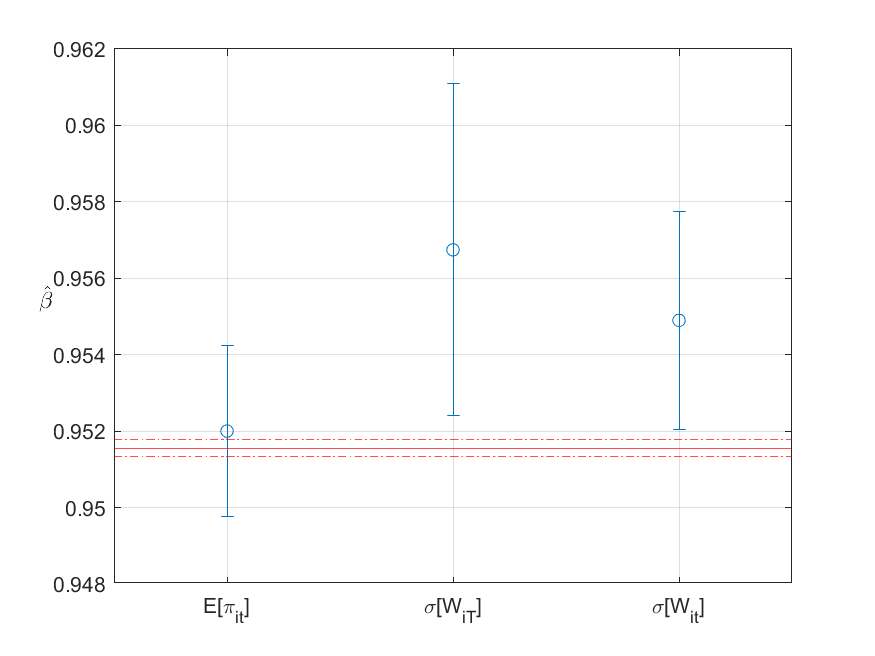
\includegraphics[width=0.45\linewidth]{Figures/moment_inclusion_check_parameterbeta.png}
    }   
    \subfloat[][Moment Inclusion for $\gamma$]{
    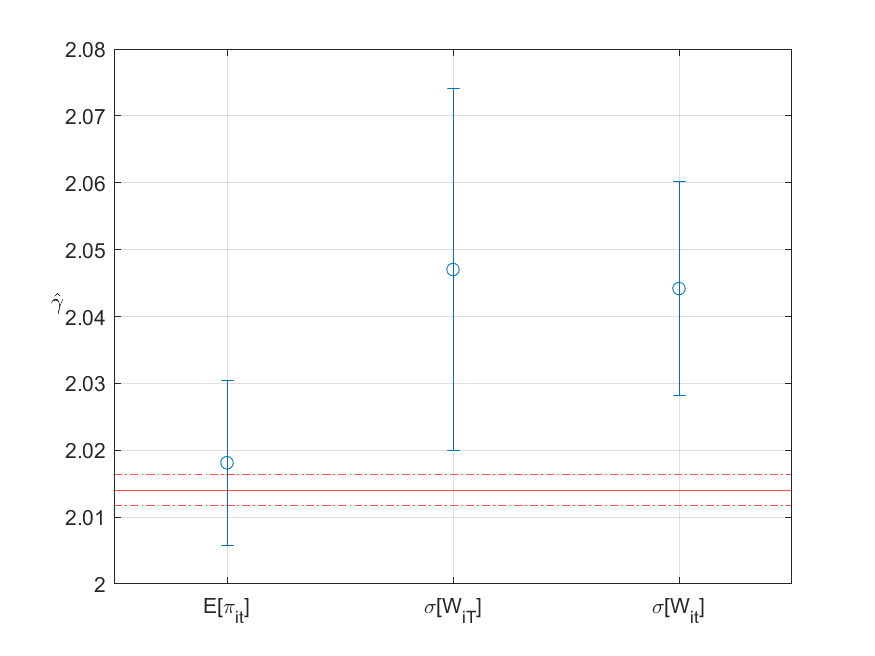
\includegraphics[width=0.45\linewidth]{Figures/moment_inclusion_check_parametergamma.png}
    }\\
    \subfloat[][Moment Inclusion for $\phi$]{
    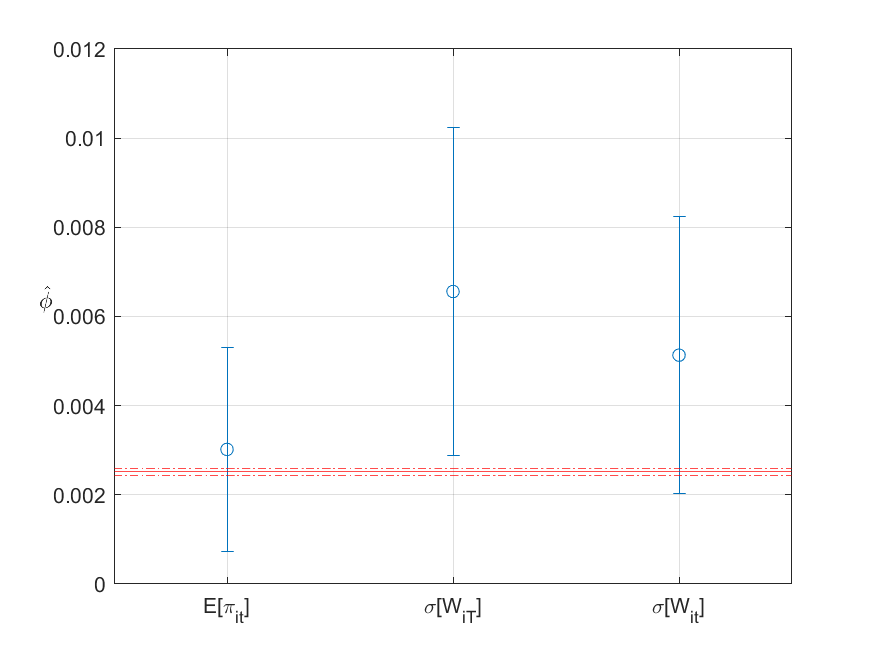
\includegraphics[width=0.45\linewidth]{Figures/moment_inclusion_check_parameterphi.png}
    }
\end{figure}